\section{Evaluation}
\label{sec:eval}

\begin{figure*}[ht!]
	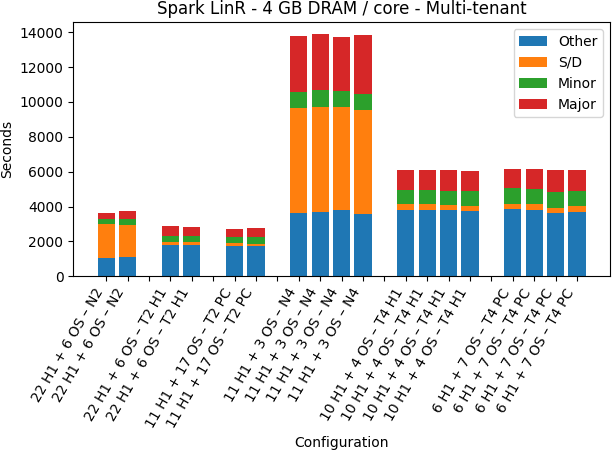
\includegraphics[width=13cm,height=6cm]{./fig/linr64.png}
    \caption{Execution time breakdown for multiple instances of
    LinearRegression using the 64 GB total DRAM setup. E.g.
    22-28-64-Native 1 indicates the first of the 2-4-8 instances that
    was run in parallel and uses 22 GB H1 - 28 GB total cgroup DRAM
    and 64 GB total DRAM for the machine.}
	\label{fig:linr64}
\end{figure*}

\begin{figure*}[ht!]
        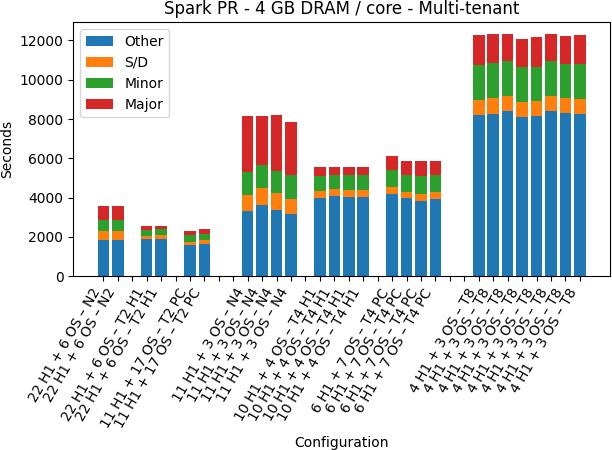
\includegraphics[width=13cm,height=6cm]{./fig/pr64.png}
    \caption{Execution time breakdown for multiple instances of
    PageRank using the 64 GB total DRAM setup. E.g. 22-28-64-Native 1
    indicates the first of the 2-4-8 instances that was run in
    parallel and uses 22 GB H1 - 28 GB total cgroup DRAM and 64 GB
    total DRAM for the machine.}
	\label{fig:pr64}
\end{figure*}

\begin{figure*}[ht!]
        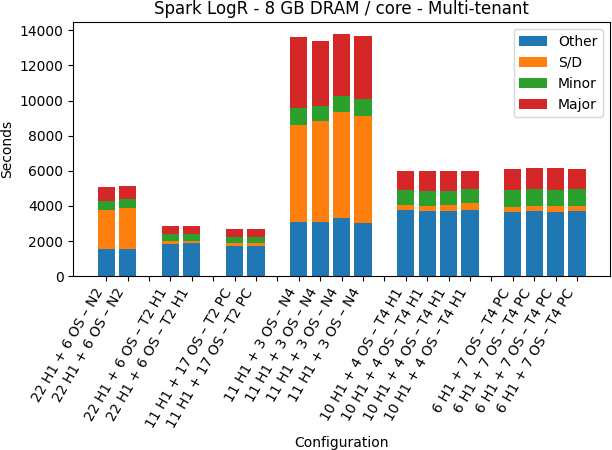
\includegraphics[width=13cm,height=6cm]{./fig/logr64.png}
    \caption{Execution time breakdown for multiple instances of
    Logistic Regression using the 64 GB total DRAM setup. E.g.
    22-28-64-Native 1 indicates the first of the 2-4-8 instances that
    was run in parallel and uses 22 GB H1 - 28 GB total cgroup DRAM
    and 64 GB total DRAM for the machine.}
	\label{fig:logr64}
\end{figure*}

\begin{figure*}[ht!]
        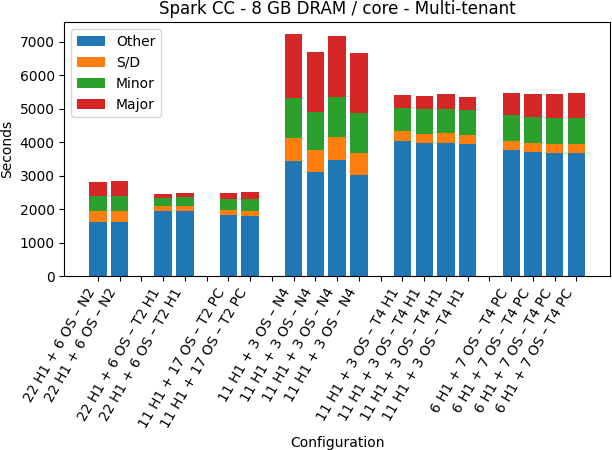
\includegraphics[width=13cm,height=6cm]{./fig/cc64.png}
    \caption{Execution time breakdown for multiple instances of
    Connected Component using the 64 GB total DRAM setup. E.g.
    22-28-64-Native 1 indicates the first of the 2-4-8 instances that
    was run in parallel and uses 22 GB H1 - 28 GB total cgroup DRAM
    and 64 GB total DRAM for the machine.}
	\label{fig:cc64}
\end{figure*}

\begin{figure*}[ht!]
        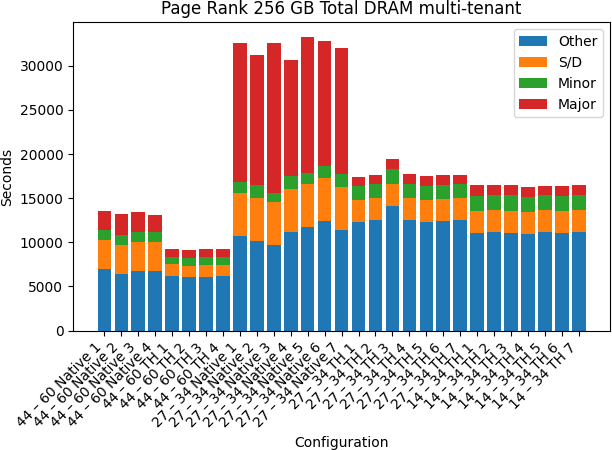
\includegraphics[width=13cm,height=6cm]{./fig/pr256.png}
    \caption{Execution time breakdown for multiple instances of
    PageRank using the 256 GB total DRAM setup. E.g. 44-60-256-Native
    1 indicates the first of the 2-4-8 instances that was run in
    parallel and uses 44 GB H1 - 60 GB total cgroup DRAM and 256 GB
    total DRAM for the machine.}
	\label{fig:pr256}
\end{figure*}

\subsection{Are GC and S/D still the main overheads of Native Spark
when running multiple spark instances and can TeraHeap increase
throughput/number of instances running by reducing these costs? What
happens with Java Heap and I/O Cache?}

Figure \ref{fig:linr64} shows the performance of multiple
Native-TeraHeap Spark instances running LinearRegression with 64 GB
dataset per instance in our 64 GB DRAM machine. Each instance of Spark
uses one executor with 8 cores per executor. Available DRAM is 56 GB
and 8 GB are left to the Operating system, resulting in 64 GB total
DRAM. Starting from the left of the graph, the first 2 bars show the
performance of Native Spark with each instance using 22 GB DRAM for H1
(Java Heap) and 6 GB for JVM Native memory and I/O cache resulting in
a total of 28 GB DRAM per instance and utilizing 56 of 64 GB total
DRAM. The next 2 bars show the performance of Native Spark with each
instance using 11 GB DRAM for H1 (Java Heap) and 17 GB for JVM Native
memory and I/O cache resulting in a total of 28 GB DRAM per instance
and utilizing 56 of 56 GB total available DRAM. The next 4 bars show
the performance of Native Spark with each instance using 11 GB DRAM
for H1 (Java Heap) and 3 GB for JVM Native memory and I/O cache
resuting in a total of 14 GB DRAM per instance and utilizing 56 of 56
GB total available DRAM. The next 2 bars show the performance of
TeraHeap Spark with each instance using 22 GB DRAM for H1 (Java Heap)
and 6 GB for JVM Native memory and I/O cache resulting in a total of
28 GB DRAM per instance and utilizing 56 of 56 GB total available
DRAM. The next 2 bars show the performance of TeraHep Spark with each
instance using 11 GB DRAM for H1 (Java Heap) and 17 GB for JVM Native
memory and I/O cache resulting in a total of 28 GB DRAM per instance
and utilizing 56 of 56 GB total available DRAM. The next 4 bars show
the performance of TeraHeap Spark with each instance using 11 GB DRAM
for H1 (Java Heap) and 3 GB for JVM Native memory and I/O cache
resuting in a total of 14 GB DRAM per instance and utilizing 56 of 56
GB total available DRAM. The next 4 bars show the performance of
TeraHeap Spark with increased PageCache and reduced H1 with each
instance using 6 GB DRAM for H1 (Java Heap) and 8 GB for JVM Native
memory and I/O cache resuting in a total of 14 GB DRAM per instance
and utilizing 56 of 56 GB total available DRAM. The next 4 bars show
the performance of TeraHeap Spark with increased PageCache and reduced
H1 with each instance using 6 GB DRAM for H1 (Java Heap) and 8 GB for
JVM Native memory and I/O cache resuting in a total of 14 GB DRAM per
instance and utilizing 56 of 56 GB total available DRAM. The last 4
bars show the performance of TeraHeap Spark with increased PageCache
and reduced H1 with each instance using 6 GB DRAM for H1 (Java Heap)
and 5 GB for JVM Native memory and I/O cache resuting in a total of 14
GB DRAM per instance and utilizing 56 of 56 GB total available DRAM.
By looking at this graph it is clear that Spark suffers by both S/D
and GC, but more specifically when it comes to LinerRegression S/D is
higher than PageRank. Furthermore we witness Major GC to increase
dramaticaly as we increase the number of Spark instances running, same
as with PageRank. These overheads are absorbed by TeraHeap. Finally
someone would prefer to have a bigger heap than I/O cache when running
LinearRegression as well.

Figure \ref{fig:pr64} shows the performance of multiple
Native-TeraHeap Spark instances running PageRank with 8 GB dataset per
instance in our 64 GB DRAM machine. Each instance of Spark uses one
executor with 8 cores per executor. Available DRAM is 56 GB and 8 GB
are left to the Operating system, resulting in 64 GB total DRAM.
Starting from the left of the graph, the first 2 bars show the
performance of Native Spark with each instance using 22 GB DRAM for H1
(Java Heap) and 6 GB for JVM Native memory and I/O cache resulting in
a total of 28 GB DRAM per instance and utilizing 56 of 64 GB total
DRAM. The next 2 bars show the performance of Native Spark with each
instance using 11 GB DRAM for H1 (Java Heap) and 17 GB for JVM Native
memory and I/O cache resulting in a total of 28 GB DRAM per instance
and utilizing 56 of 56 GB total available DRAM. The next 4 bars show
the performance of Native Spark with each instance using 11 GB DRAM
for H1 (Java Heap) and 3 GB for JVM Native memory and I/O cache
resuting in a total of 14 GB DRAM per instance and utilizing 56 of 56
GB total available DRAM. The next 4 bars show the performance of
TeraHeap Spark with increased PageCache and reduced H1 with each
instance using 9 GB DRAM for H1 (Java Heap) and 5 GB for JVM Native
memory and I/O cache resuting in a total of 14 GB DRAM per instance
and utilizing 56 of 56 GB total available DRAM. The next 2 bars show
the performance of TeraHeap Spark with each instance using 22 GB DRAM
for H1 (Java Heap) and 6 GB for JVM Native memory and I/O cache
resulting in a total of 28 GB DRAM per instance and utilizing 56 of 56
GB total available DRAM. The next 2 bars show the performance of
TeraHep Spark with each instance using 11 GB DRAM for H1 (Java Heap)
and 17 GB for JVM Native memory and I/O cache resulting in a total of
28 GB DRAM per instance and utilizing 56 of 56 GB total available
DRAM. The next 4 bars show the performance of TeraHeap Spark with each
instance using 11 GB DRAM for H1 (Java Heap) and 3 GB for JVM Native
memory and I/O cache resuting in a total of 14 GB DRAM per instance
and utilizing 56 of 56 GB total available DRAM. The next 4 bars show
the performance of TeraHeap Spark with increased PageCache and reduced
H1 with each instance using 6 GB DRAM for H1 (Java Heap) and 8 GB for
JVM Native memory and I/O cache resuting in a total of 14 GB DRAM per
instance and utilizing 56 of 56 GB total available DRAM. The last 8
bars show the performance of TeraHeap Spark with each instance using 4
GB DRAM for H1 (Java Heap) and 3 GB for JVM Native memory and I/O
cache resuting in a total of 7 GB DRAM per instance and utilizing 56
of 56 GB total available DRAM.  By looking at this graph it is clear
that Spark suffers by both S/D and GC, but more specifically when it
comes to PageRank we witness Major GC to increase dramaticaly as we
increase the number of Spark instances running. These overheads are
absorbed by TeraHeap. TeraHeap also scales to 8 instances while Native
can't because it runs out of memory. Finally someone would prefer to
have a bigger heap than I/O cache when running PageRank.

Figure \ref{fig:logr64} shows the performance of multiple Native-TeraHeap
Spark instances running LogisticRegression with 8 GB dataset per
instance in our 64 GB DRAM machine. Each instance of Spark uses one
executor with 8 cores per executor. Available DRAM is 56 GB and 8 GB
are left to the Operating system, resulting in 64 GB total DRAM.
Starting from the left of the graph, the first 2 bars show the
performance of Native Spark with each instance using 22 GB DRAM for H1
(Java Heap) and 6 GB for JVM Native memory and I/O cache resulting in
a total of 28 GB DRAM per instance and utilizing 56 of 64 GB total
DRAM. The next 2 bars show the performance of Native Spark with each
instance using 11 GB DRAM for H1 (Java Heap) and 17 GB for JVM Native
memory and I/O cache resulting in a total of 28 GB DRAM per instance
and utilizing 56 of 56 GB total available DRAM. The next 4 bars show
the performance of Native Spark with each instance using 11 GB DRAM
for H1 (Java Heap) and 3 GB for JVM Native memory and I/O cache
resuting in a total of 14 GB DRAM per instance and utilizing 56 of 56
GB total available DRAM. The next 4 bars show the performance of
TeraHeap Spark with increased PageCache and reduced H1 with each
instance using 9 GB DRAM for H1 (Java Heap) and 5 GB for JVM Native
memory and I/O cache resuting in a total of 14 GB DRAM per instance
and utilizing 56 of 56 GB total available DRAM. The next 2 bars show
the performance of TeraHeap Spark with each instance using 22 GB DRAM
for H1 (Java Heap) and 6 GB for JVM Native memory and I/O cache
resulting in a total of 28 GB DRAM per instance and utilizing 56 of 56
GB total available DRAM. The next 2 bars show the performance of
TeraHep Spark with each instance using 11 GB DRAM for H1 (Java Heap)
and 17 GB for JVM Native memory and I/O cache resulting in a total of
28 GB DRAM per instance and utilizing 56 of 56 GB total available
DRAM. The next 4 bars show the performance of TeraHeap Spark with each
instance using 11 GB DRAM for H1 (Java Heap) and 3 GB for JVM Native
memory and I/O cache resuting in a total of 14 GB DRAM per instance
and utilizing 56 of 56 GB total available DRAM. The next 4 bars show
the performance of TeraHeap Spark with increased PageCache and reduced
H1 with each instance using 6 GB DRAM for H1 (Java Heap) and 8 GB for
JVM Native memory and I/O cache resuting in a total of 14 GB DRAM per
instance and utilizing 56 of 56 GB total available DRAM.  By looking
at this graph it is clear that Spark suffers by both S/D and GC, but
more specifically when it comes to LogisticRegression we witness S/D
to increase dramaticaly as we increase the number of Spark instances
running. These overheads are absorbed by TeraHeap. Finally someone
would prefer to have a bigger heap than I/O cache when running
LogisticRegression.

Figure \ref{fig:cc64} shows the performance of multiple Native-TeraHeap
Spark instances running ConnectedComponent with 8 GB dataset per
instance in our 64 GB DRAM machine. Each instance of Spark uses one
executor with 8 cores per executor. Available DRAM is 56 GB and 8 GB
are left to the Operating system, resulting in 64 GB total DRAM.
Starting from the left of the graph, the first 2 bars show the
performance of Native Spark with each instance using 22 GB DRAM for H1
(Java Heap) and 6 GB for JVM Native memory and I/O cache resulting in
a total of 28 GB DRAM per instance and utilizing 56 of 64 GB total
DRAM. The next 2 bars show the performance of Native Spark with each
instance using 11 GB DRAM for H1 (Java Heap) and 17 GB for JVM Native
memory and I/O cache resulting in a total of 28 GB DRAM per instance
and utilizing 56 of 56 GB total available DRAM. The next 4 bars show
the performance of Native Spark with each instance using 11 GB DRAM
for H1 (Java Heap) and 3 GB for JVM Native memory and I/O cache
resuting in a total of 14 GB DRAM per instance and utilizing 56 of 56
GB total available DRAM. The next 2 bars show the performance of
TeraHeap Spark with each instance using 22 GB DRAM for H1 (Java Heap)
and 6 GB for JVM Native memory and I/O cache resulting in a total of
28 GB DRAM per instance and utilizing 56 of 56 GB total available
DRAM. The next 2 bars show the performance of TeraHep Spark with each
instance using 11 GB DRAM for H1 (Java Heap) and 17 GB for JVM Native
memory and I/O cache resulting in a total of 28 GB DRAM per instance
and utilizing 56 of 56 GB total available DRAM. The next 4 bars show
the performance of TeraHeap Spark with each instance using 11 GB DRAM
for H1 (Java Heap) and 3 GB for JVM Native memory and I/O cache
resuting in a total of 14 GB DRAM per instance and utilizing 56 of 56
GB total available DRAM. The next 4 bars show the performance of
TeraHeap Spark with increased PageCache and reduced H1 with each
instance using 6 GB DRAM for H1 (Java Heap) and 8 GB for JVM Native
memory and I/O cache resuting in a total of 14 GB DRAM per instance
and utilizing 56 of 56 GB total available DRAM.  By looking at this
graph it is clear that Spark suffers by both S/D and GC, but more
specifically when it comes to ConnectedComponent we witness Major GC
to increase dramaticaly as we increase the number of Spark instances
running. These overheads are absorbed by TeraHeap. Finally someone
would prefer to have a bigger heap than I/O cache when running
ConnectedComponent.

Figure \ref{fig:pr256} shows the performance of multiple Native-TeraHeap
Spark instances running PageRank with 32 GB dataset per instance in
our 256 GB DRAM machine. Each instance of Spark uses one executor with
8 cores per executor. Available DRAM is 240 GB and 16 GB are left to
the Operating system, resulting in 256 GB total DRAM. Starting from
the left of the graph, the first 4 bars show the performance of Native
Spark with each instance using 44 GB DRAM for H1 (Java Heap) and 16 GB
for JVM Native memory and I/O cache resulting in a total of 60 GB DRAM
per instance and utilizing 240 of 256 GB total DRAM. The next 6 bars
show the performance of Native Spark with each instance using 32 GB
DRAM for H1 (Java Heap) and 8 GB for JVM Native memory and I/O cache
resulting in a total of 40 GB DRAM per instance and utilizing 240 of
240 GB total available DRAM. The next 7 bars show the performance of
Native Spark with each instance using 27 GB DRAM for H1 (Java Heap)
and 7 GB for JVM Native memory and I/O cache resuting in a total of 34
GB DRAM per instance and utilizing 240 of 240 GB total available DRAM.
The next 7 bars show the performance of TeraHeap Spark with each
instance using 27 GB DRAM for H1 (Java Heap) and 7 GB for JVM Native
memory and I/O cache resuting in a total of 34 GB DRAM per instance
and utilizing 240 of 240 GB total available DRAM. The last 7 bars show
the performance of Native Spark with each instance using 14 GB DRAM
for H1 (Java Heap) and 20 GB for JVM Native memory and I/O cache
resuting in a total of 34 GB DRAM per instance and utilizing 240 of
240 total DRAM. By looking at this graph it is clear that Spark
suffers by both S/D and GC, but more specifically when it comes to
PageRank we witness Major GC to increase dramaticaly as we increase
the number of Spark instances running. These overheads are absorbed by
TeraHeap. Finally someone would prefer to have a bigger heap than I/O
cache when running PageRank.

\subsection{Is the CPU utilization of the server incresing
accordingly to throughput?}

\begin{figure*}[ht!]
        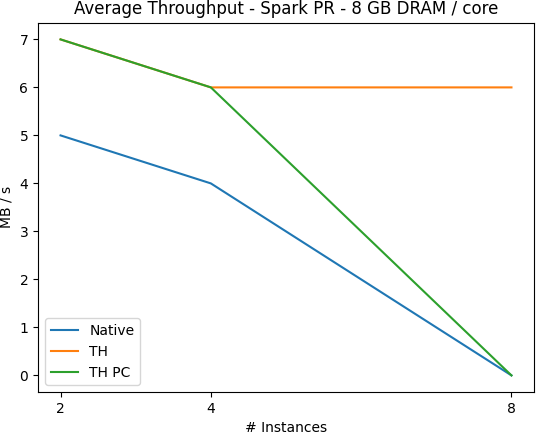
\includegraphics[width=13cm,height=6cm]{./fig/PR_64_THR.png}
    \caption{Page Rank 64 GB DRAM setup Native and TeraHeap throughput
    as the number of instances increases. Configurations starting with
    N denote a run with Native instances of Spark and with T with
    TeraHeap. H1 is a run with the memory budget configured to contain
    a bigger size for H1 than PageCache and PC the opposite. E.g. T2
    PC is a run of 2 concurrent TeraHeap instances with exactly the
    same configuration.}
	\label{fig:pr_64_thr}
\end{figure*}

\begin{figure*}[ht!]
        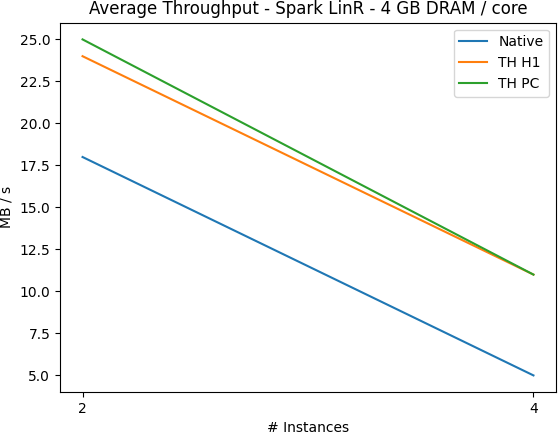
\includegraphics[width=13cm,height=6cm]{./fig/LINR_64_THR.png}
    \caption{Linear Regression 64 GB DRAM setup Native and TeraHeap
    throughput as the number of instances increases. Configurations
    starting with N denote a run with Native instances of Spark and
    with T with TeraHeap. H1 is a run with the memory budget
    configured to contain a bigger size for H1 than PageCache and PC
    the opposite. E.g. T2 PC is a run of 2 concurrent TeraHeap
    instances with exactly the same configuration.}
	\label{fig:linr_64_thr}
\end{figure*}

\begin{figure*}[ht!]
        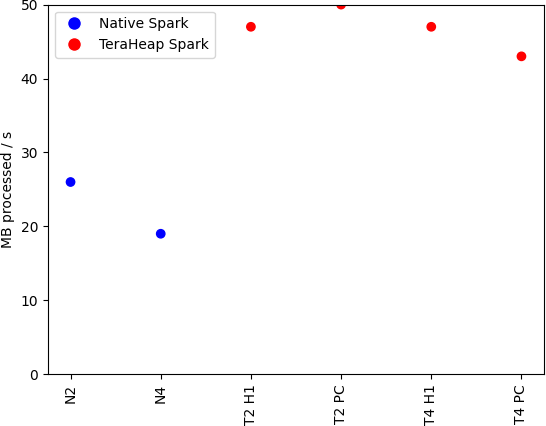
\includegraphics[width=13cm,height=6cm]{./fig/LOGR_64_THR.png}
    \caption{Logistic Regression 64 GB DRAM setup Native and TeraHeap
    throughput as the number of instances increases. Configurations
    starting with N denote a run with Native instances of Spark and
    with T with TeraHeap. H1 is a run with the memory budget
    configured to contain a bigger size for H1 than PageCache and PC
    the opposite. E.g. T2 PC is a run of 2 concurrent TeraHeap
    instances with exactly the same configuration.}
	\label{fig:logr_64_thr}
\end{figure*}

\begin{figure*}[ht!]
        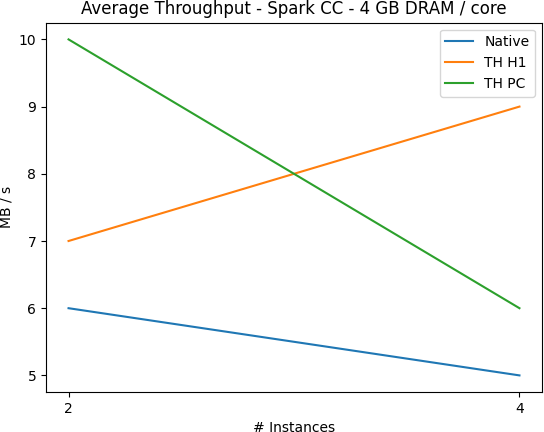
\includegraphics[width=13cm,height=6cm]{./fig/CC_64_THR.png}
    \caption{Connected Component 64 GB DRAM setup Native and TeraHeap
    throughput as the number of instances increases.Configurations
    starting with N denote a run with Native instances of Spark and
    with T with TeraHeap. H1 is a run with the memory budget
    configured to contain a bigger size for H1 than PageCache and PC
    the opposite. E.g. T2 PC is a run of 2 concurrent TeraHeap
    instances with exactly the same configuration. }
	\label{fig:cc_64_thr}
\end{figure*}

\begin{figure*}[ht!]
        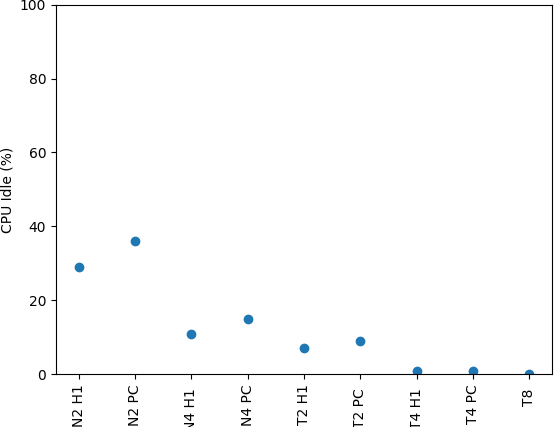
\includegraphics[width=13cm,height=6cm]{./fig/PR_64_IDLE.png}
    \caption{Page Rank 64 GB DRAM setup Native and TeraHeap idle CPU
    as the number of instances increases. Configurations starting with
    N denote a run with Native instances of Spark and with T with
    TeraHeap. H1 is a run with the memory budget configured to contain
    a bigger size for H1 than PageCache and PC the opposite. E.g. T2
    PC is a run of 2 concurrent TeraHeap instances with exactly the
    same configuration.}
	\label{fig:pr_64_idle}
\end{figure*}

\begin{figure*}[ht!]
        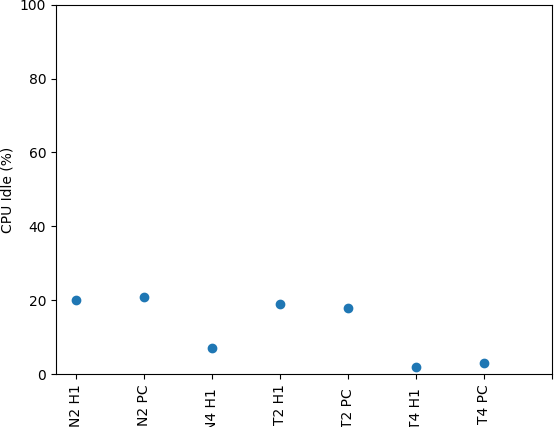
\includegraphics[width=13cm,height=6cm]{./fig/LINR_64_IDLE.png}
    \caption{Linear Regression 64 GB DRAM setup Native and TeraHeap
    idle CPU as the number of instances increases. Configurations
    starting with N denote a run with Native instances of Spark and
    with T with TeraHeap. H1 is a run with the memory budget
    configured to contain a bigger size for H1 than PageCache and PC
    the opposite. E.g. T2 PC is a run of 2 concurrent TeraHeap
    instances with exactly the same configuration.}
	\label{fig:linr_64_idle}
\end{figure*}

\begin{figure*}[ht!]
        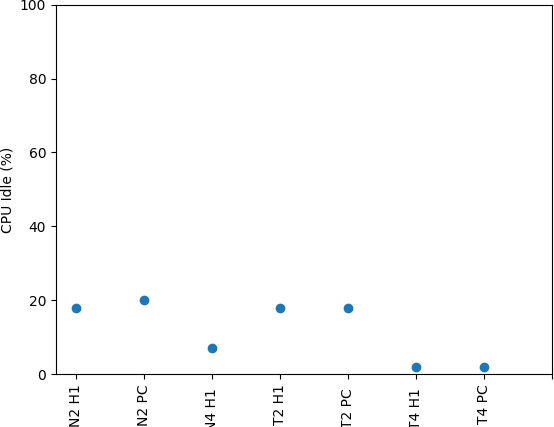
\includegraphics[width=13cm,height=6cm]{./fig/LOGR_64_IDLE.png}
    \caption{Logistic Regression 64 GB DRAM setup Native and TeraHeap
    idle CPU as the number of instances increases. Configurations
    starting with N denote a run with Native instances of Spark and
    with T with TeraHeap. H1 is a run with the memory budget
    configured to contain a bigger size for H1 than PageCache and PC
    the opposite. E.g. T2 PC is a run of 2 concurrent TeraHeap
    instances with exactly the same configuration.}
	\label{fig:logr_64_idle}
\end{figure*}

\begin{figure*}[ht!]
        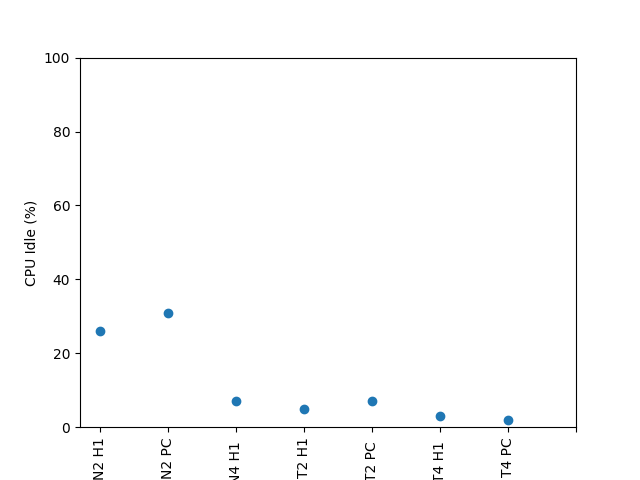
\includegraphics[width=13cm,height=6cm]{./fig/CC_64_IDLE.png}
    \caption{Connected Component 64 GB DRAM setup Native and TeraHeap
    idle CPU as the number of instances increases. Configurations
    starting with N denote a run with Native instances of Spark and
    with T with TeraHeap. H1 is a run with the memory budget
    configured to contain a bigger size for H1 than PageCache and PC
    the opposite. E.g. T2 PC is a run of 2 concurrent TeraHeap
    instances with exactly the same configuration.}
	\label{fig:cc_64_idle}
\end{figure*}

By looking at figures \ref{fig:pr_64_thr}, \ref{fig:linr_64_thr},
\ref{fig:logr_64_thr} and \ref{fig:cc_64_thr} we see that Native
Spark's throughput decreases as the number of colocated
instances-executors increase in the server. The main goal for
colocating tasks is to increase the CPU utilization and achieve better
throughput as effectively as possible as if running each instance
isolated. While Native Spark fails to provide scalability, TH Spark
achieves nearly double the throughput of Native Spark and is also able
to scale beyond 4 instances.

Figures \ref{fig:pr_64_idle}, \ref{fig:linr_64_idle},
\ref{fig:logr_64_idle} and \ref{fig:cc_64_idle}  show the percentage
of idle CPU while the number of colocated instances grows. CPU idle
should decrease in this particular concept and that is something
proven in the figure. In PageRank graph we notice TeraHeap with 2
instances achieving less idle CPU percentage than Native Spark with 4
instances.

\subsection{Detailed synopsis of multi-instances evaluation. What
happens with monetary cost across different cloud platforms?}

\begin{table}[t!]
  \centering
  \caption{Page Rank synopsis table. Configurations starting
    with N denote a run with Native instances of Spark and with T with
    TeraHeap. H1 is a run with the memory budget configured to contain
    a bigger size for H1 than PageCache and PC the opposite.}
  \label{tab:linr_table}
        \resizebox{19cm}{!}{
        \begin{tabular}{|c|c|c|c|c|c|c|c|c|c|c|c|c|}
      \hline
\textbf{Conf.} & \textbf{H1 Size/I} & \textbf{Memory/I} & \textbf{Total Mem.} & \textbf{\#I} & \textbf{Exec. Time} & \textbf{CPU Idle} & \textbf{Total MB Proc.} & \textbf{MB/s} & \textbf{MB/s/I} & \textbf{Cost AWS \$} & \textbf{Cost GCP \$} & \textbf{Cost Azure \$} \\
        \hline
    N2 - small & 22 & 28 & 64 & 2 & 3563 & 29 & 16980 & 5 & 2 & 0.6 & 0.58 & 0.67 \\
    N4 - small & 11 & 14 & 64 & 4 & 8195 & 11 & 33960 & 4 & 1 & 1.8 & 1.74 & 2.01 \\
    T2 H1 – small & 22 & 28 & 64 & 2 & 2545 & 7 & 16980 & 7 & 3 & 0.6 & 0.58 & 0.67 \\
    T2 PC – small & 11 & 28 & 64 & 2 & 2385 & 9 & 16980 & 7 & 4 & 0.6 & 0.58 & 0.67 \\
    T4 H1 – small & 11 & 14 & 64 & 4 & 5554 & 1 & 33960 & 6 & 2 & 1.2 & 1.16 & 1.34 \\
    T4 PC – small & 6 & 14 & 64 & 4 & 5880 & 1 & 33960 & 6 & 2 & 1.2 & 1.16 & 1.34 \\
    N8 – small & 4 & 7 & 64 & 8 & OOM & ** & 0 & 0 & 0 & *** & *** & *** \\
    T8 – small & 4 & 7 & 64 & 8 & 12305 & 0 & 67920 & 6 & 1 & 2.4 & 2.32 & 2.68 \\
    N4 - big & 44 & 60 & 256 & 4 & 13542 & 15 & 135872 & 10 & 3 & 6.4 & *** & *** \\
    T4 – big & 48 & 60 & 256 & 4 & 9284 & 5 & 135782 & 16 & 4 \\      
	\hline
     \end{tabular}%
        }
\end{table}


\begin{table}[t!]
  \centering
  \caption{Linear Regression synopsis table. Configurations starting
    with N denote a run with Native instances of Spark and with T with
    TeraHeap. H1 is a run with the memory budget configured to contain
    a bigger size for H1 than PageCache and PC the opposite.}
  \label{tab:linr_table}
        \resizebox{19cm}{!}{
        \begin{tabular}{|c|c|c|c|c|c|c|c|c|c|c|c|c|}
      \hline
\textbf{Conf.} & \textbf{H1 Size/I} & \textbf{Memory/I} & \textbf{Total Mem.} & \textbf{\#I} & \textbf{Exec. Time} & \textbf{CPU Idle} & \textbf{Total MB Proc.} & \textbf{MB/s} & \textbf{MB/s/I} & \textbf{Cost AWS \$} & \textbf{Cost GCP \$} & \textbf{Cost Azure \$} \\
	\hline 
      N2 & 22 & 28 & 64 & 2 & 3745 & 20 & 134896 & 37 & 18 & 0.6 & 0.58 & 0.67 \\ 
      N4 & 11 & 14 & 64 & 4 & 13874 & 7 & 269792 & 20 & 5 & 2.4 & 2.32 & 2.01 \\
      T2 H1 & 22 & 28 & 64 & 2 & 2891 & 19 & 134896 & 48 & 24 & 0.6 & 0.58 & 0.67 \\
      T2 PC & 11 & 28 & 64 & 2 & 2747 & 18 & 134896 & 49 & 25 & 0.6 & 0.58 & 0.67 \\
      T4 H1 & 11 & 14 & 64 & 4 & 6075 & 2 & 269792 & 44 & 11 & 1.2 & 1.16 & 1.34 \\
      T4 PC & 6 & 14 & 64 & 4 & 6176 & 3 & 269792 & 44 & 11 & 1.2 & 1.16 & 1.34 \\ 
      \hline
     \end{tabular}%
	}
\end{table}

\begin{table}[t!]
  \centering
  \caption{Logistic Regression synopsis table. Configurations starting
    with N denote a run with Native instances of Spark and with T with
    TeraHeap. H1 is a run with the memory budget configured to contain
    a bigger size for H1 than PageCache and PC the opposite.}
  \label{tab:logr_table}
	\resizebox{19cm}{!}{
	\begin{tabular}{|c|c|c|c|c|c|c|c|c|c|c|c|c|}
      \hline
\textbf{Conf.} & \textbf{H1 Size/I} & \textbf{Memory/I} & \textbf{Total Mem.} & \textbf{\#I} & \textbf{Exec. Time} & \textbf{CPU Idle} & \textbf{Total MB Proc.} & \textbf{MB/s} & \textbf{MB/s/I} & \textbf{Cost AWS \$} & \textbf{Cost GCP \$} & \textbf{Cost Azure \$} \\
      \hline
      N2 & 22 & 28 & 64 & 2 & 5127 & 18 & 133348 & 26 & 13 & 1.2 & 1.16 & 0.67 \\
      N4 & 11 & 14 & 64 & 4 & 13730 & 7 & 266696 & 19 & 5 & 2.4 & 2.32 & 2.68 \\
      T2 H1 & 22 & 28 & 64 & 2 & 2861 & 18 & 133348 & 47 & 24 & 0.6 & 0.58 & 0.67 \\
      T2 PC & 11 & 28 & 64 & 2 & 2683 & 18 & 133348 & 50 & 25 & 0.6 & 0.58 & 0.67 \\
      T4 H1 & 10 & 14 & 64 & 4 & 5712 & 2 & 266696 & 47 & 12 & 1.2 & 1.16 & 1.34 \\
      T4 PC & 6 & 14 & 64 & 4 & 6138 & 2 & 266696 & 43 & 10 & 1.2 & 1.16 & 1.34 \\
      \hline
     \end{tabular}%
	}
\end{table}

\begin{table}[t!]
  \centering
  \caption{Connected Component synopsis table. Configurations starting
    with N denote a run with Native instances of Spark and with T with
    TeraHeap. H1 is a run with the memory budget configured to contain
    a bigger size for H1 than PageCache and PC the opposite.}
  \label{tab:cc_table}
        \resizebox{19cm}{!}{
        \begin{tabular}{|c|c|c|c|c|c|c|c|c|c|c|c|c|}
      \hline
\textbf{Conf.} & \textbf{H1 Size/I} & \textbf{Memory/I} & \textbf{Total Mem.} & \textbf{\#I} & \textbf{Exec. Time} & \textbf{CPU Idle} & \textbf{Total MB Proc.} & \textbf{MB/s} & \textbf{MB/s/I} & \textbf{Cost AWS \$} & \textbf{Cost GCP \$} & \textbf{Cost Azure \$} \\
	\hline
      N2 & 22 & 28 & 64 & 2 & 2958 & 26 & 16980 & 6 & 3 & 0.6 & 0.58 & 0.67 \\
      N4 & 11 & 14 & 64 & 4 & 7231 & 7 & 33960 & 5 & 3 & 1.8 & 1.74 & 2.01 \\
      T2 H1 & 22 & 28 & 64 & 2 & 2526 & 5 & 16980 & 7 & 4 & 0.6 & 0.58 & 0.67 \\
      T2 PC & 11 & 28 & 64 & 2 & 2519 & 7 & 16980 & 7 & 4 & 0.6 & 0.58 & 0.67 \\
      T4 H1 & 11 & 14 & 64 & 4 & 5439 & 3 & 33960 & 6 & 3 & 1.2 & 0.58 & 0.67 \\
      T4 PC & 6 & 14 & 64 & 4 & 5487 & 2 & 33960 & 6 & 3 & 1.2 & 1.16 & 1.34 \\
      \hline
     \end{tabular}%
	}
\end{table}

Tables \ref{fig:pr_table}, \ref{tab:linr_table}, \ref{tab:logr_table}
and \ref{tab:cc_table} show a detailed synopsis of the performance and
AWS, GCP and Azure costs of deploying multiple instances of Spark
using both techniques. Each setup is run using 2 different amounts for
H1 (80 and 40\%). While the number of instances increases TeraHeap
appears to maintain throughput while Native Spark has significant
throughput decrease. In several occassions, if we compare Native's to
TeraHeap's throughput we notice TeraHeap having more than 100\%
increase compared to Native. In PageRank's 64 DB DRAM setup TeraHeap
manages to scale to 8 instances while Native Spark runs out of memory.
Furthermore when looking at the PageRank table it becomes clear that
TeraHeap achieves a higher CPU utilization, because of the S/D
elimination and less I/O. Despite TeraHeap's better performance, the
total time taken for all instances to complete surpasses the time it
would take to run the same number of single isolated instances one
after the other. This means that in order to achieve better
performance we would need a scheduling policy to decide H1 and
PageCache amount for each workload running. This is something
discussed in the next section. Moreover, regarding the monetary cost
across different cloud platforms such as AWS EC2 (Amazon Web Services
Cloud), Google Cloud Platform (GCP) and Microsoft Azure, we witness
that all providers offer a similar cost for identical machines. As
seen by the tables, taking into account that we have an hourly cost,
TeraHeap seems to be the obvious choice for running Spark workloads
and save money, because it is able to offer more scalability to the
user by freeing memory in order to increase CPU utilization and
increase throughput. 
